\documentclass{article}

\usepackage[norsk]{babel}
\usepackage[margin=1.5in]{geometry}
\usepackage{graphicx}
\usepackage{wrapfig}

\usepackage{caption}
\usepackage{subcaption}

\usepackage{listings}
\usepackage{listings-rust}
\usepackage{color}
\usepackage{xcolor}
\definecolor{light-gray}{gray}{0.95}
\newcommand{\code}[1]{\colorbox{light-gray}{\texttt{#1}}}

\definecolor{dkgreen}{rgb}{0,0.6,0}
\definecolor{gray}{rgb}{0.5,0.5,0.5}
\definecolor{mauve}{rgb}{0.58,0,0.82}

\lstset{
  language=Rust,
  aboveskip=3mm,
  belowskip=3mm,
  columns=flexible,
  basicstyle={\small\ttfamily},
  numbers=left,
  numberstyle=\color{gray},
  keywordstyle=\color{blue},
  commentstyle=\color{dkgreen},
  stringstyle=\color{mauve},
  breaklines=true,
  breakatwhitespace=true,
  tabsize=4
}

\title{IDATT2104 - Datakom Oblig 1}
\author{Jakob Grønhaug (jakobkg@stud.ntnu.no)}

\begin{document}
\maketitle

\tableofcontents

\section{P3: Sockets, TCP, HTTP og tråder}

\subsection{Enkel tjener/klient}

Til denne oppgaven har jeg skrevet en enkel tjener som lytter på port 3000 etter koblinger fra klienter, og svarer på enkle regnestykker. Med Netcat som klient ser interaksjon med denne tjeneren slik ut:

\begin{figure}[ht]
    \centering
    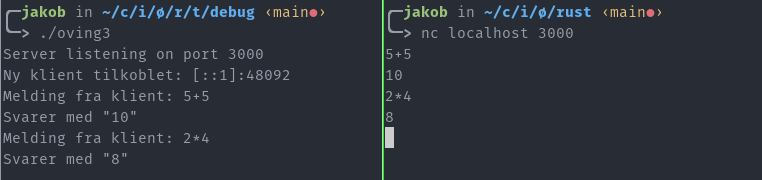
\includegraphics[width=.8\linewidth]{illustrasjoner/P3-enkel-terminal.png}
    \caption{Enkel tjener som utfører regnestykker, brukt med Netcat som klient}
\end{figure}

Dette tjener-programmet er basert på \code{TcpListener}-klassen fra Rusts standardbibliotek\footnote{https://doc.rust-lang.org/std/net/struct.TcpListener.html}, som oppretter en \textbf{TCP}-kobling over IP. Når programmet kun kjører lokalt hos meg er det spesifikt IPv6 som brukes, som kan sees i pakkefangsten i følgende figur (adresse \texttt{::1} i stedet for \texttt{127.0.0.1}). Siden dette programmet bruker TCP foregår det et handshake (SYN, SYN/ACK, ACK) når en klient kobles til tjeneren, og et lignende handshake (FIN, FIN/ACK, ACK) når koblingen lukkes fordi enten klienten eller tjeneren avsluttes. Dette kan også sees i en pakkefangst med Wireshark:

\begin{figure}[ht]
    \centering
    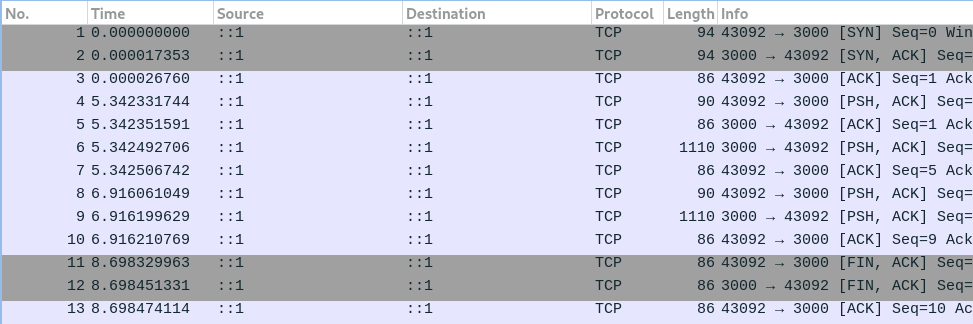
\includegraphics[width=.8\linewidth]{illustrasjoner/P3-enkel-capture.png}
    \caption{Pakkefangst av tjener med kun en klient}
    \label{fig2}
\end{figure}

Siden koblingen bruker TCP er all kommunisjon gjort i parvise pakker, der den ene pakken er at en av partene sender data i en pakke og den andre parten (dersom alt går som det skal) svarer med en ACK-pakke for å bekrefte at dataen ble mottatt. I dette programmet er kommunikasjonen på formen regnestykke/svar, så forventet kommunikasjon for et enkelt regnestykke er klient-data\rightarrow tjener-ack\rightarrow tjener-data\rightarrow klient-ack. Dette kan for eksempel sees i figur 2, der pakkene 4-7 viser en slik frem-og-tilbake mellom klienten og tjeneren.

Merk også at svaret fra tjeneren er betydelig større enn forespørselen fra klienten. Dette skyldes at jeg på tjener-siden oppretter en buffer på 1kB (1024 byte), putter dataen som tjeneren ønsker å sende inn i denne bufferen og sender hele bufferen av gårde. En bedre løsning ville vært å kun sende den delen av bufferen som faktisk inneholder data, men den løsningen som er brukt her fungerer også selv om den har enorm overhead.
Den relevante delen av koden der denne bufferen opprettes og sendes uten å sjekke hvor mye av bufferen som faktisk er nyttig data er:

\begin{lstlisting}
    // Tømmer respons-bufferen før behandling
    responsebuf = [0; 1024];
    
    // Behandler forespørselen og genererer svar vha funksjonsobjektet response_fn som legges i responsebuf
    (self.response_fn)(message.into_owned(), &mut responsebuf);
    
    // Sender responsebuf tilbake, avslutter om sendingen feiler av noen grunn
    if let Err(e) = socket.write_all(&responsebuf).await {
        eprintln!("Problem ved skrivning til socket: {e:?}");
        return;
    }
\end{lstlisting}

Merk spesielt linje 2 der bufferen fylles med 1024 bytes med \texttt{0x00}, og linje 8 der denne bufferen sendes av gårde gjennom nettverket uten at den forkortes fra sin fulle størrelse på 1024 bytes på noen måte. På klient-siden er Netcat flinkere til å ikke sende en drøss med unødvendig data, forskjellen kan sees veldig tydelig i pakkevisningen i Wireshark, se figur \ref{fig:pakkesammenligning} nedenfor.

\begin{figure}[ht]
    \centering
    \begin{subfigure}[t]{.45\linewidth}
        \centering
        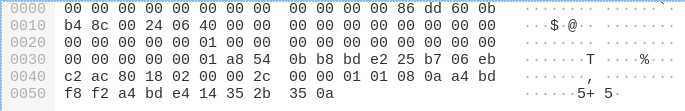
\includegraphics[width=\linewidth]{illustrasjoner/P3-fra-netcat.png}
        \caption{En pakke sendt fra Netcat med data "\texttt{5+5}"}
    \end{subfigure}
    \hfill
    \begin{subfigure}[t]{.45\linewidth}
        \centering
        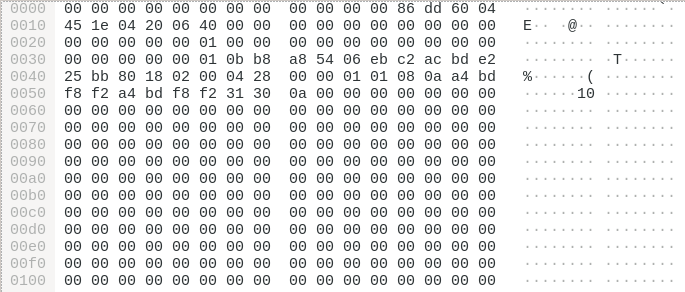
\includegraphics[width=\linewidth]{illustrasjoner/P3-fra-tjener.png}
        \caption{En pakke sendt fra tjeneren med data "\texttt{10}", fulgt av i overkant av tusen null-bytes}
    \end{subfigure}

    \caption{Sammenligninger av pakker sendt fra Netcat og fra tjener-programmet}
    \label{fig:pakkesammenligning}
\end{figure}

\subsection{Flere samtidige klienter}

For å utvide tjener-programmet har jeg brukt Rust-biblioteket Tokio\footnote{https://docs.rs/tokio/1.25.0/tokio/} for å enklere opprette en tråd for hver klient som kobles til tjeneren. På denne måten kan flere klienter kommunisere med tjeneren til samme tid uten å måtte vente på tur eller oppleve nevneverdig ventetid fra tjeneren mottar en forespørsel til den faktisk behandles. Det er fortsatt Rusts \texttt{TcpListener} og de tilhørende typene som ligger i bunnen av programmet, og dermed fortsatt TCP som benyttes.
I følgende skjermbilde fra Wireshark kan man se to separate SYN\rightarrow SYN/ACK\rightarrow ACK-sekvenser og to separate FIN\rightarrow FIN/ACK\rightarrow ACK-sekvenser, for hhv. oppkobling og nedkobling mellom klient og tjener.

\begin{figure}[h]
    \begin{subfigure}{.48\linewidth}
        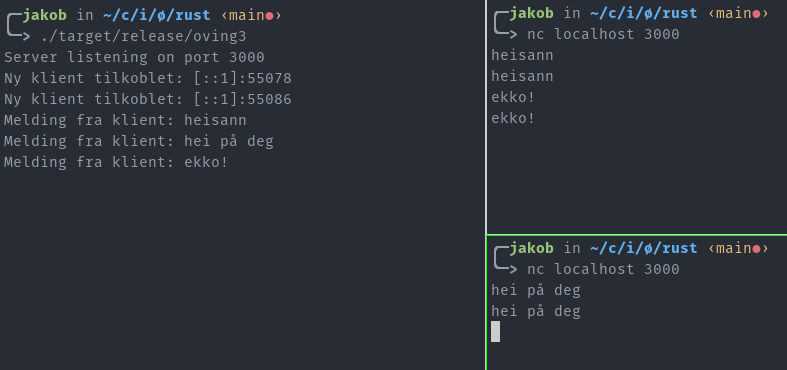
\includegraphics[width=\linewidth]{illustrasjoner/P3-flere-terminal.png}
        \caption{Terminal med en tjener og to klienter}
    \end{subfigure}
    \hfill
    \begin{subfigure}{.48\linewidth}
        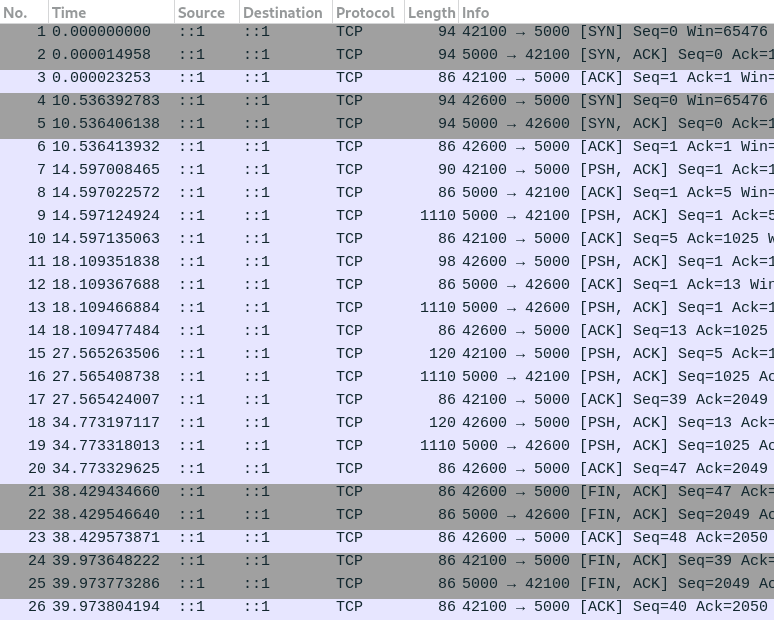
\includegraphics[width=\linewidth]{illustrasjoner/P3-flere-capture.png}
        \caption{Pakkefangst av en tjener og to klienter som gjør oppkobling, noen forespørsler hver, og nedkobling}
    \end{subfigure}
    \caption{Kjøring og pakkefangst av en tjener med to samtidige klienter}
\end{figure}

I denne varianten av tjeneren er koden som behandler forespørsler og genererer svar endret fra å lese og utføre regnestykker til å bare kopiere dataen fra den mottatte forespørselen til bufferen som sendes i retur (en ekko-tjener). Selve koden som behandler sending av responser fra tjeneren til klientene er den samme som i den forrige oppgaven, så problemet med overdrevent store svar-pakker opptrer her også på samme måte som før (se f.eks. pakke 9 og 13). Den eneste forskjellen i håndteringen av klienter er at det nå opprettes en ny tråd for hver klient, som håndterer sin klientens forespørsler. Dette er oppnådd ved å pakke inn den relevante koden i en \code{loop \{...\}}, og bruke \code{tokio::spawn(...)} til å opprette en ny tråd hver gang en oppkoblingsforespørsel mottas.

\subsection{Web med nettleser som klient}

Takket være litt lur modularisering av tjener-programmet er all koden som behandler oppkobling og samtidighet gjenbrukt fra forrige oppgave, og en ny funksjon som leser HTTP-forespørsler og genererer et HTML-dokument som spesifisert i oppgaveteksten er alt som trengs av ny kode. Denne nye funksjonen behandler alle innkommende forespørsler likt og anerkjenner ikke muligheten for at noen skulle kunne ønske seg noe annet enn et HTML-dokument i svar på forespørselen sin, men fungerer likefullt mer enn godt nok til denne oppgaven. Siden all kode som har med nettverk/sockets å gjøre er gjenbrukt er det fremdeles TCP som er i bruk. Det er verdt å merke seg at siden det ikke er noen kryptering eller sikkerhet som SSL eller TLS inne i bildet kan denne tjeneren kun HTTP, ikke HTTPS.

\begin{figure}[h]
    \centering
    \begin{subfigure}{.48\linewidth}
        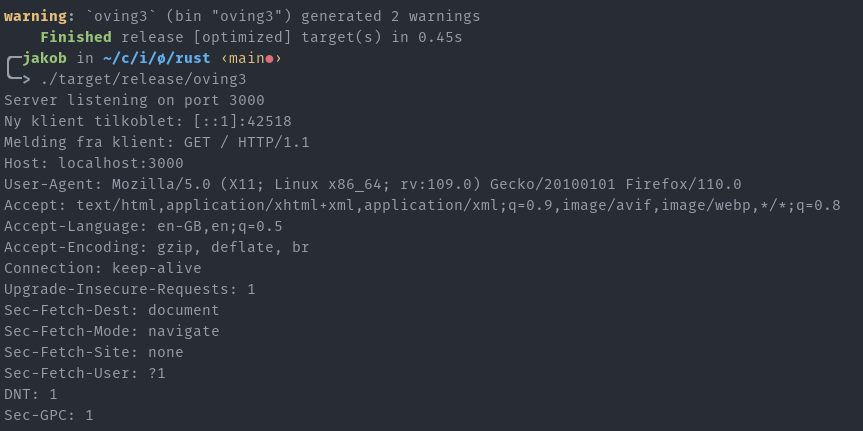
\includegraphics[width=\linewidth]{illustrasjoner/P3-web-tjener.png}
        \caption{Terminal med web-tjener}
    \end{subfigure}
    \hfill
    \begin{subfigure}{.48\linewidth}
        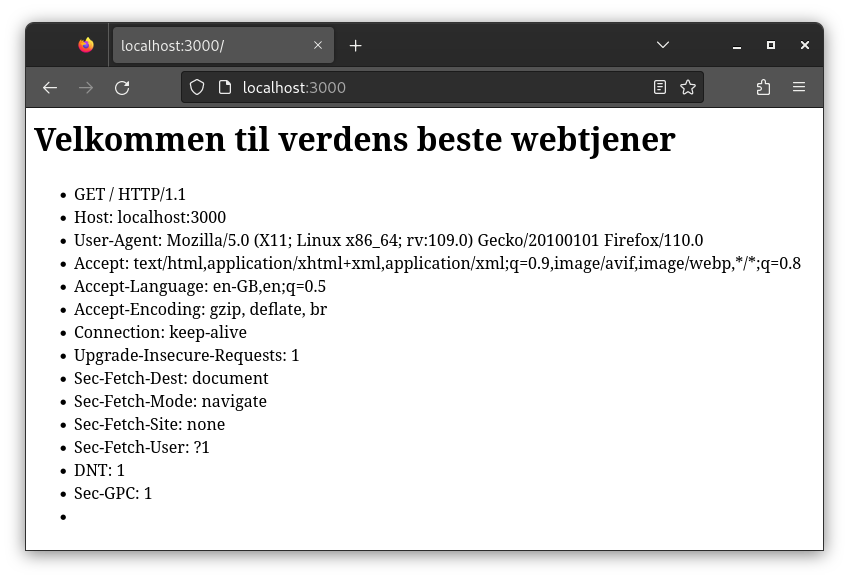
\includegraphics[width=\linewidth]{illustrasjoner/P3-web-klient.png}
        \caption{Svaret på forespørselen fra (a), vist i Firefox}
    \end{subfigure}

    \begin{subfigure}{.8\linewidth}
        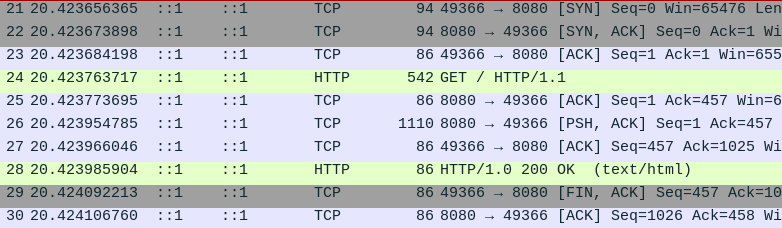
\includegraphics[width=\linewidth]{illustrasjoner/P3-web-capture.png}
        \caption{Pakkene som går frem og tilbake mellom nettleser og webtjener. Pakker fra port 49366 stammer fra nettleseren, og pakker fra port 8080 stammer fra tjeneren.}
    \end{subfigure}
    \caption{Web-tjener, klient og pakkefangst}
\end{figure}

Denne gangen er det implementert HTTP, en protokoll som Wireshark faktisk forstår og kan vise noe mer informasjon om! De tidligere oppgavene har kun vært tekst over TCP uten noen ordentlig protokoll, som begrenser hvor mye metadata og nyttig info Wireshark kan vise om pakkene som går frem og tilbake. Nå som det er gyldige HTTP-pakker som sendes kan Wireshark vise litt mer info basert på protokollen. Se f.eks. pakkefangsten i figuren over, der pakke 24 og 28 er HTTP-pakker med hhv \texttt{GET / HTTP/1.1} og \texttt{HTTP/1.0 200 OK} med respons-body av typen \texttt{text/html}. All denne infoen Wireshark fremhever er hentet fra headerne til pakkene som sendes frem og tilbake.

\begin{wrapfigure}{r}{.5\linewidth}
    \centering
    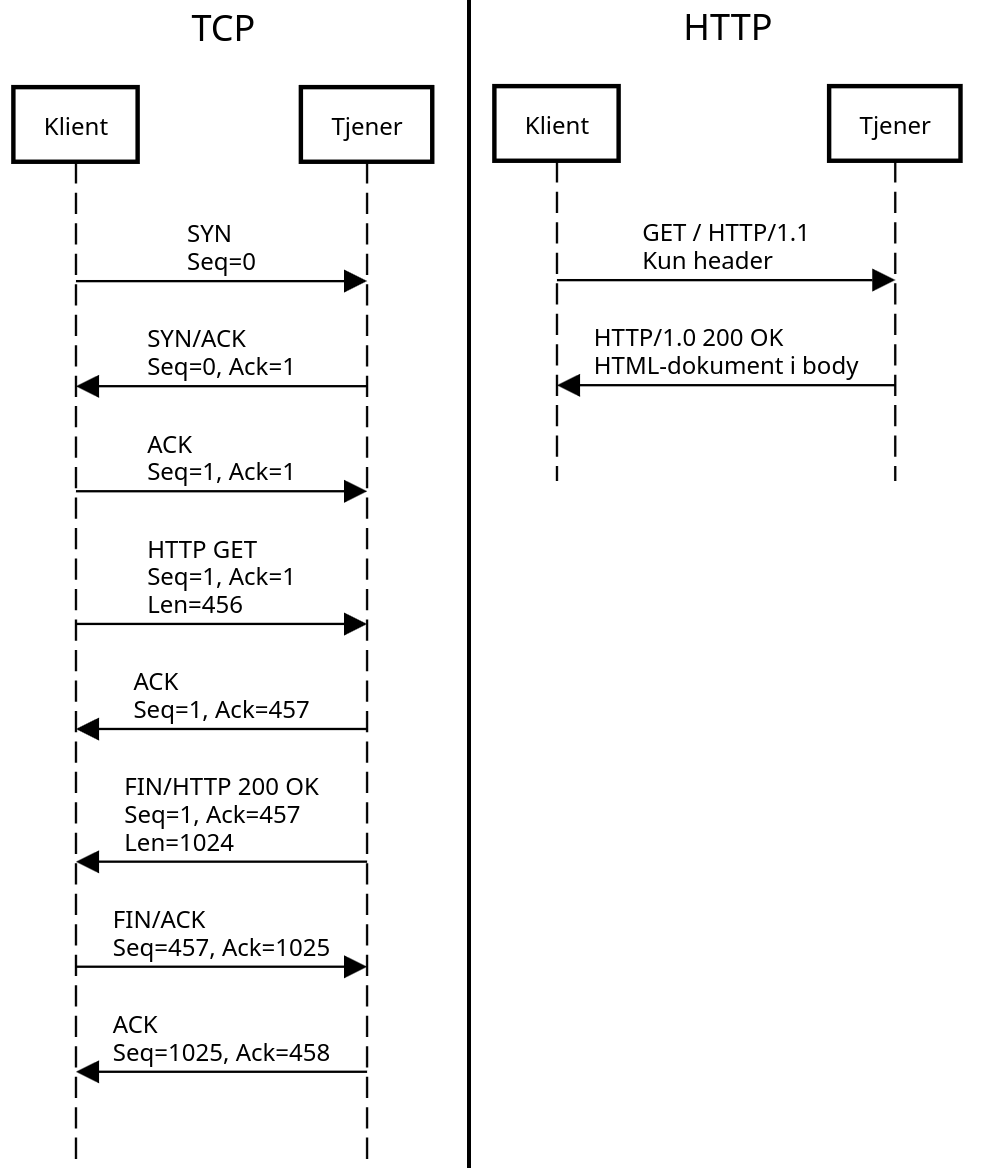
\includegraphics[width=.8\linewidth]{illustrasjoner/P3-web-sekvens.png}
    \caption{Sekvensdiagram som viser den samme trafikken slik den ser ut på transportlaget og på applikasjonslaget}
\end{wrapfigure}

Siden deler av HTTP er implementert kan vi nå se på denne pakkeutvekslingen i flere lag, og se at det er en betydelig enklere interaksjon som foregår på applikasjonslaget (HTTP) enn på transportlaget (TCP).
Der transportlaget håndterer oppkobling, nedkobling og synkronisering, trenger applikasjonslaget bare å sende meldinger frem og tilbake mellom klient og tjener uten å måtte dobbeltsjekke om trafikken faktisk kommer frem eller ikke.

Det er denne typen abstraksjoner som gjør lagmodellen for nettverk så nyttig, det at man på applikasjonslaget kan arbeide med en antagelse om at de underliggende lagene i modellen gjør jobben sin uten at man trenger å tenke på dem 

\section{P4: UDP, TLS}

\subsection{UDP-kalkulator}

I denne oppgaven er kalkulator-programmet fra tidligere endret til å kommunisere over UDP i stedet for TCP. Dette fjerner en betydelig andel overhead fra kommunikasjonen og forenkler programmeringen noe, siden koblingen mellom klient og tjener ikke lenger er tilstandsfull og dermed ikke trenger handshakes, oppkobling eller nedkobling for å fungere. Data bare sendes av gårde, og programmet trenger ikke lenger ta stilling til om den blir mottatt og kvittert hos mottakeren. Denne gangen er det klassen \code{std::net::UdpSocket} fra Rusts standardbibliotek som brukes for å sende/motta pakker gjennom en gitt port.

\begin{figure}[h]
    \centering
    \begin{subfigure}{.45\linewidth}
        \centering
        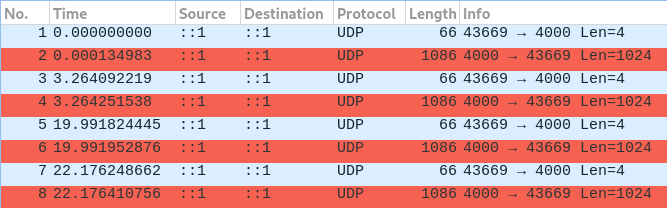
\includegraphics[width=\linewidth]{illustrasjoner/P4-UDP-capture.png}
        \caption[short]{Pakkefangst av UDP-trafikk, pakker fra klient i blått og pakker fra tjener i rødt}
    \end{subfigure}
    \hfill
    \begin{subfigure}{.45\linewidth}
        \centering
        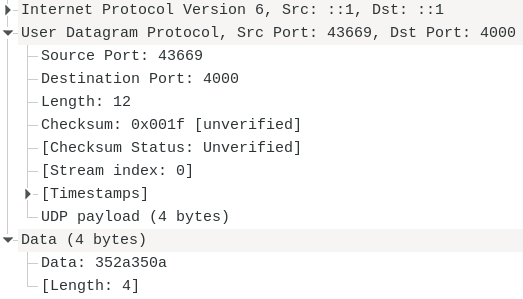
\includegraphics[width=\linewidth]{illustrasjoner/P4-UDP-header.png}
        \caption[short]{UDP-header, som vist i Wireshark}
    \end{subfigure}
    \caption{Wireshark-visning av UDP-pakker}
\end{figure}

Som kan sees av headerne fra nettverkslaget er dette lokal trafikk (både til og fra IP ::1, som er IPv6-adressen til \texttt{localhost}), og av headerne på UDP-pakken kan det leses at tjeneren er tilknyttet port 4000 mens klienten er tilknyttet port 43669.

\subsection{TLS}


\end{document}